\section{Introduction to Parallel Programming Concepts}
\makesubcontentsslides

%%% Intro to parallelism
\subsection{A Concise Introduction to Parallelism}

\begin{frame}
  \begin{block}{What is Parallelism?}\pause
  \begin{itemize}
    \item Doing more than one thing at a time.
    \item The simultaneous use of multiple compute resources to solve a 
computational problem.
  \end{itemize}
  \end{block}
\end{frame}

\begin{frame}
  \begin{block}{Parallelism}\pause
    \begin{center}
    \begin{minipage}{.46\textwidth}
    \begin{block}{\centering Serial Programming}
      \begin{center}
      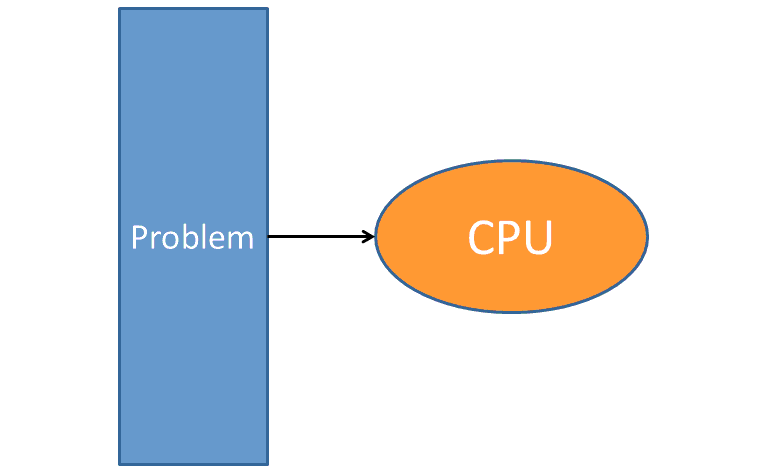
\includegraphics[width=.975\textwidth]{../common/pics/parallelism1}
      \end{center}
      \end{block}
    \end{minipage}
    \hspace{.15cm}
    \begin{minipage}{.46\textwidth}
    \begin{block}{\centering Parallel Programming}
      \begin{center}
      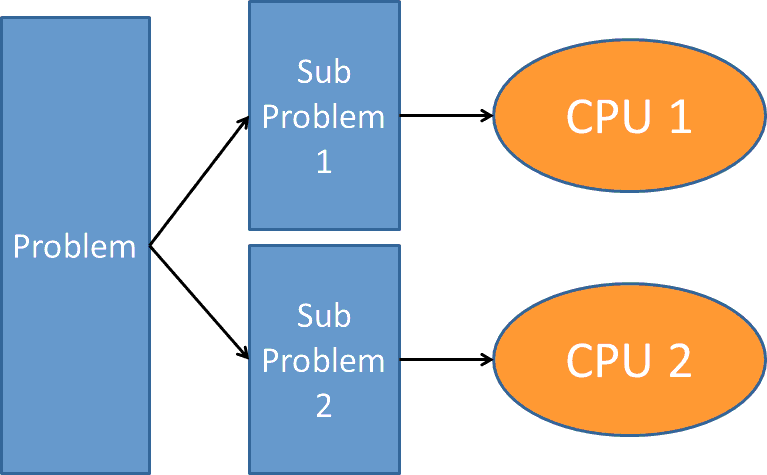
\includegraphics[width=.975\textwidth]{../common/pics/parallelism2}
      \end{center}
      \end{block}
    \end{minipage}
    \end{center}
  \end{block}
\end{frame}

\begin{frame}
  \begin{block}{Parallelism}\pause
    \begin{center}
    \begin{minipage}{.46\textwidth}
    \begin{block}{Serial Programming}
      \begin{center}
      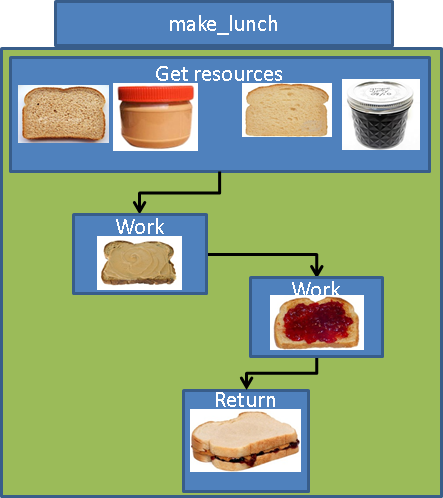
\includegraphics[width=.975\textwidth]{../common/pics/analogy_serial}
      \end{center}
      \end{block}
    \end{minipage}
    \hspace{.15cm}
    \begin{minipage}{.46\textwidth}
    \begin{block}{Parallel Programming}
      \begin{center}
      
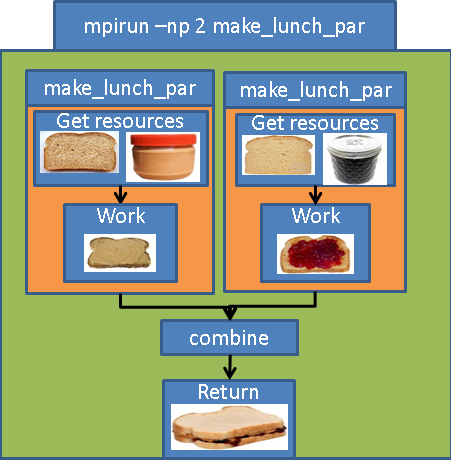
\includegraphics[height=5.45cm,width=.975\textwidth]{../common/pics/analogy_parallel}
      \end{center}
      \end{block}
    \end{minipage}
    \end{center}
  \end{block}
\end{frame}


\begin{frame}
  \begin{block}{Kinds of Parallelism}\pause
    \begin{itemize}[<+-|alert@+>]
      \item \emph{Data Parallelism}:  Data is distributed
      \item \emph{Task Parallelism}:  Tasks are distributed
  \end{itemize}
  (This is a gross oversimplification)
  \end{block}
\end{frame}


\begin{frame}
  \begin{block}{pbdR Paradigms:  Data Parallelism}
  Data parallelism:
  \begin{itemize}[<+-|alert@+>]
   \item No one processor/node owns all the data.
   \item Processors own local pieces of a (conceptually) larger, global object
  \end{itemize}
  
  Task parallelism:
  \begin{itemize}
    \item (Usually) Applying different tasks to the same data.
  \end{itemize}
  \end{block}
\end{frame}


\begin{frame}
  \begin{block}{Data vs Task Parallelism}\pause
    \begin{center}
    \begin{minipage}{.46\textwidth}
    \begin{block}{\centering Data Parallelism}
      \begin{center}
      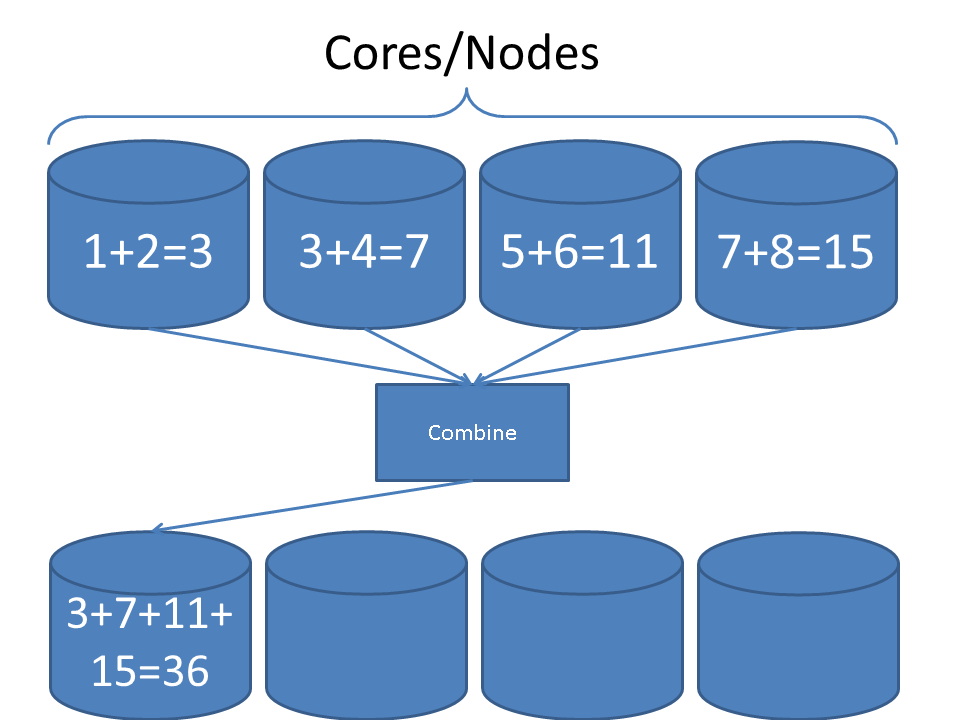
\includegraphics[width=.975\textwidth]{../common/pics/parallelism_data}
      \end{center}
      \end{block}
    \end{minipage}
    \hspace{.15cm}
    \begin{minipage}{.46\textwidth}
    \begin{block}{\centering Task Parallelism}
      \begin{center}
      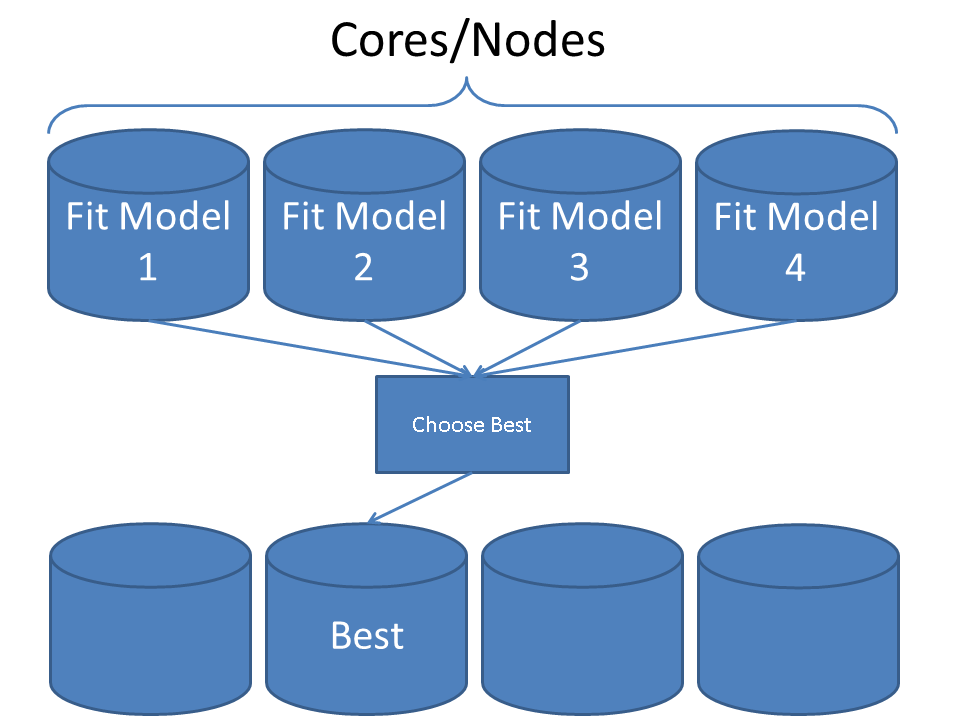
\includegraphics[width=.975\textwidth]{../common/pics/parallelism_task}
      \end{center}
      \end{block}
    \end{minipage}
    \end{center}
  \end{block}
\end{frame}




% \subsection{Common Terminology}


\begin{frame}
  \begin{block}{Parallel Programming Vocabulary:  Difficulty in Parallelism}
  \begin{enumerate}[<+-|alert@+>]
    \item \emph{Implicit parallelism}:  Parallel details hidden from user
    \item \emph{Explicit parallelism}:  Some assembly required\dots
    \item \emph{Embarrassingly Parallel}:  Also called \emph{loosely coupled}.  
Obvious how to make parallel; lots of independence in computations.
    \item \emph{Tightly Coupled}:  Opposite of embarrassingly parallel; lots of 
dependence in computations.
  \end{enumerate}  
  \end{block}
\end{frame}


\begin{frame}
  \begin{block}{Speedup}
  \begin{itemize}
    \item \emph{Wallclock Time}:  Time of the clock on the wall from start to 
finish
    \item \emph{Speedup}:  unitless measure of improvement; more is better.
  \begin{align*}
   S_{n_1, n_2} =  \frac{\text{Run time for } n_1 \text{ cores}}{\text{Run time 
for } n_2 \text{ cores}}
  \end{align*}
  \begin{itemize}
    \item   $n_1$ is often taken to be 1
    \item In this case, comparing parallel algorithm to serial algorithm
  \end{itemize}
  \end{itemize}
  \end{block}
\end{frame}


\begin{frame}
  \begin{block}{Speedup}
   \begin{center}
    \begin{minipage}{.475\textwidth}
    \begin{block}{Good Speedup}
      \centering
      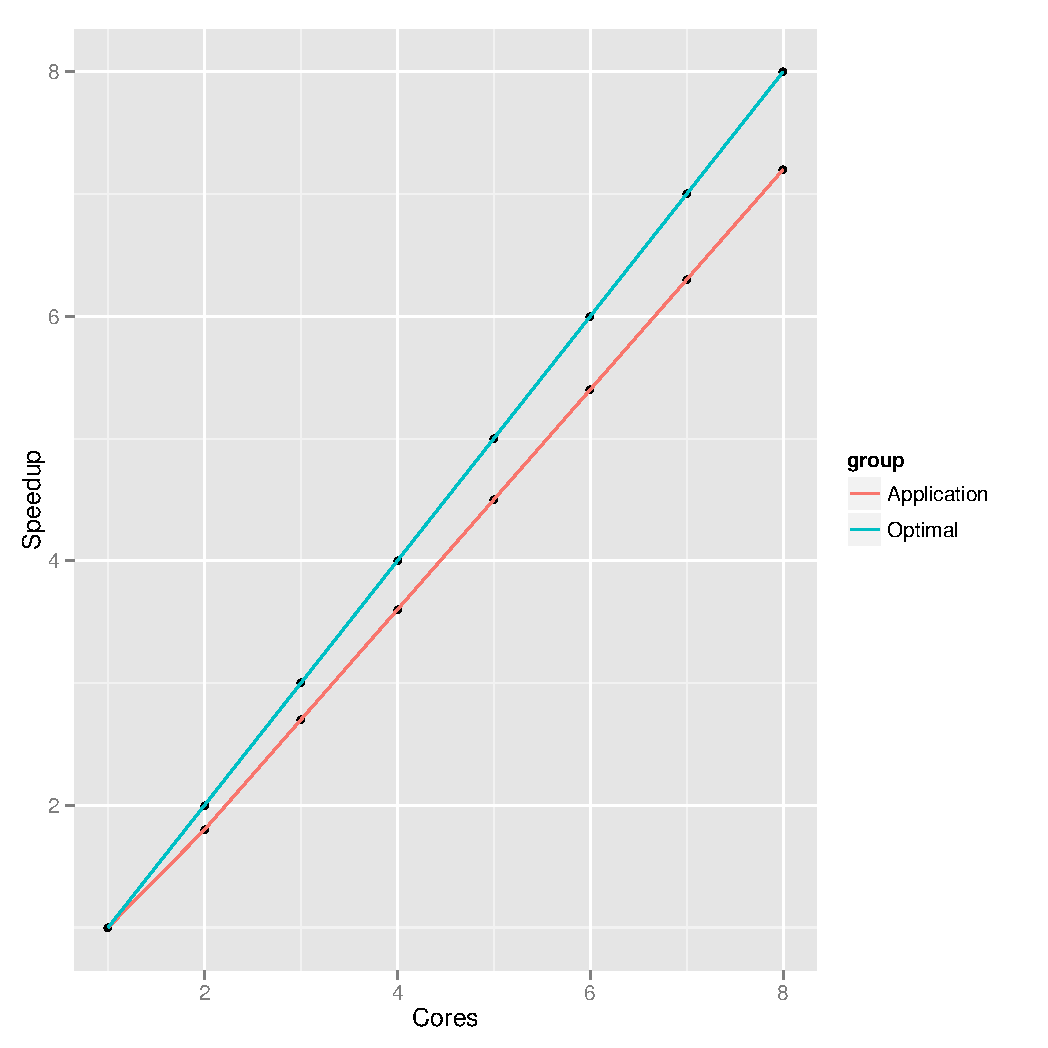
\includegraphics[width=.95\textwidth]{../common/pics/scale_good}
    \end{block}
    \end{minipage}
    \hspace{.1cm}
    \begin{minipage}{.475\textwidth}
    \begin{block}{Bad Speedup}
      \centering
      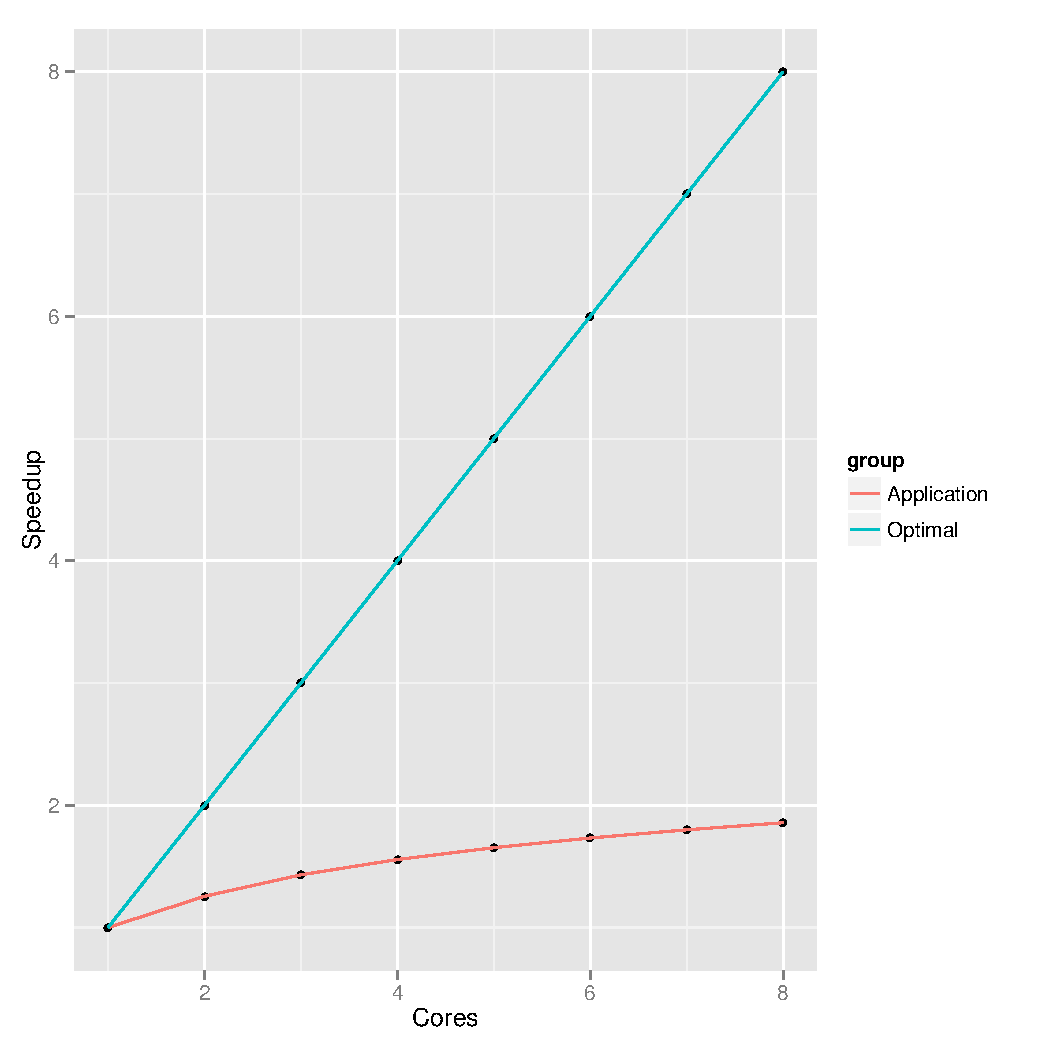
\includegraphics[width=.95\textwidth]{../common/pics/scale_bad}
    \end{block}
    \end{minipage}
    \end{center}
    \end{block}
\end{frame}


\begin{frame}
  \begin{block}{Shared and Distributed Memory Machines}
   \begin{center}
    \begin{minipage}{.475\textwidth}
    \begin{block}{Shared Memory}
     Direct access to read/change memory (one node) \vspace{.3cm} \ 
      \begin{center}
      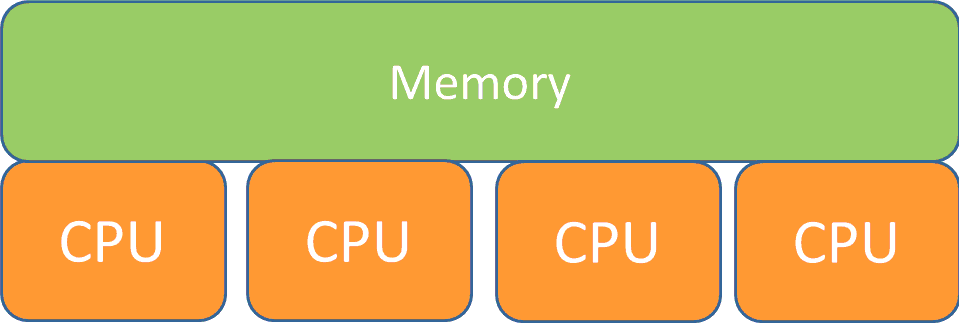
\includegraphics[width=.95\textwidth]{../common/pics/arch_shared}
      \end{center}
      \vspace{.3cm} \
    \end{block}
    \end{minipage}
    \hspace{.1cm}
    \begin{minipage}{.475\textwidth}
    \begin{block}{Distributed}
    No direct access to read/change memory (many nodes); requires communication
      \begin{center}
      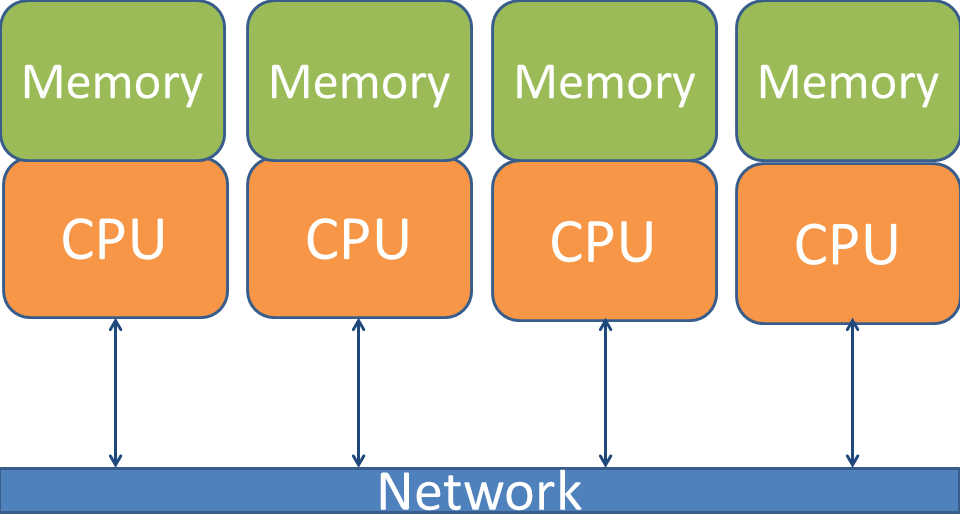
\includegraphics[width=.95\textwidth]{../common/pics/arch_distributed}
      \end{center}
    \end{block}
    \end{minipage}
    \end{center}
    \end{block}
\end{frame}


\begin{frame}
  \begin{block}{Shared and Distributed Memory Machines}
   \begin{center}
    \begin{minipage}[t]{.47\textwidth}
    \begin{block}{Shared Memory Machines}
    \begin{center}
    Thousands of cores\\[.2cm]
    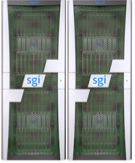
\includegraphics[scale=.65]{../common/pics/nautilus}\\
    {\tiny \emph{Nautilus}, University of Tennessee\\1024 cores \\4 TB RAM\\}
    \end{center}
    \end{block}
    \end{minipage}
    \hspace{.1cm}
    \begin{minipage}[t]{.47\textwidth}
    \begin{block}{Distributed Memory Machines}
    \begin{center}
    Hundreds of thousands of cores\\[.2cm]
    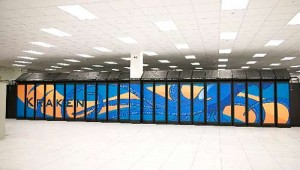
\includegraphics[width=.95\textwidth]{../common/pics/kraken}\\
    {\tiny \emph{Kraken}, University of Tennessee\\ 112,896 cores \\147 TB 
RAM\\}
    \end{center}
    \end{block}
    \end{minipage}
    \end{center}
    \end{block}
\end{frame}


\section{Shared Memory Parallel Packages in R}
\makesubcontentsslides

\begin{frame}{R Interfaces to Low-Level Native Tools}
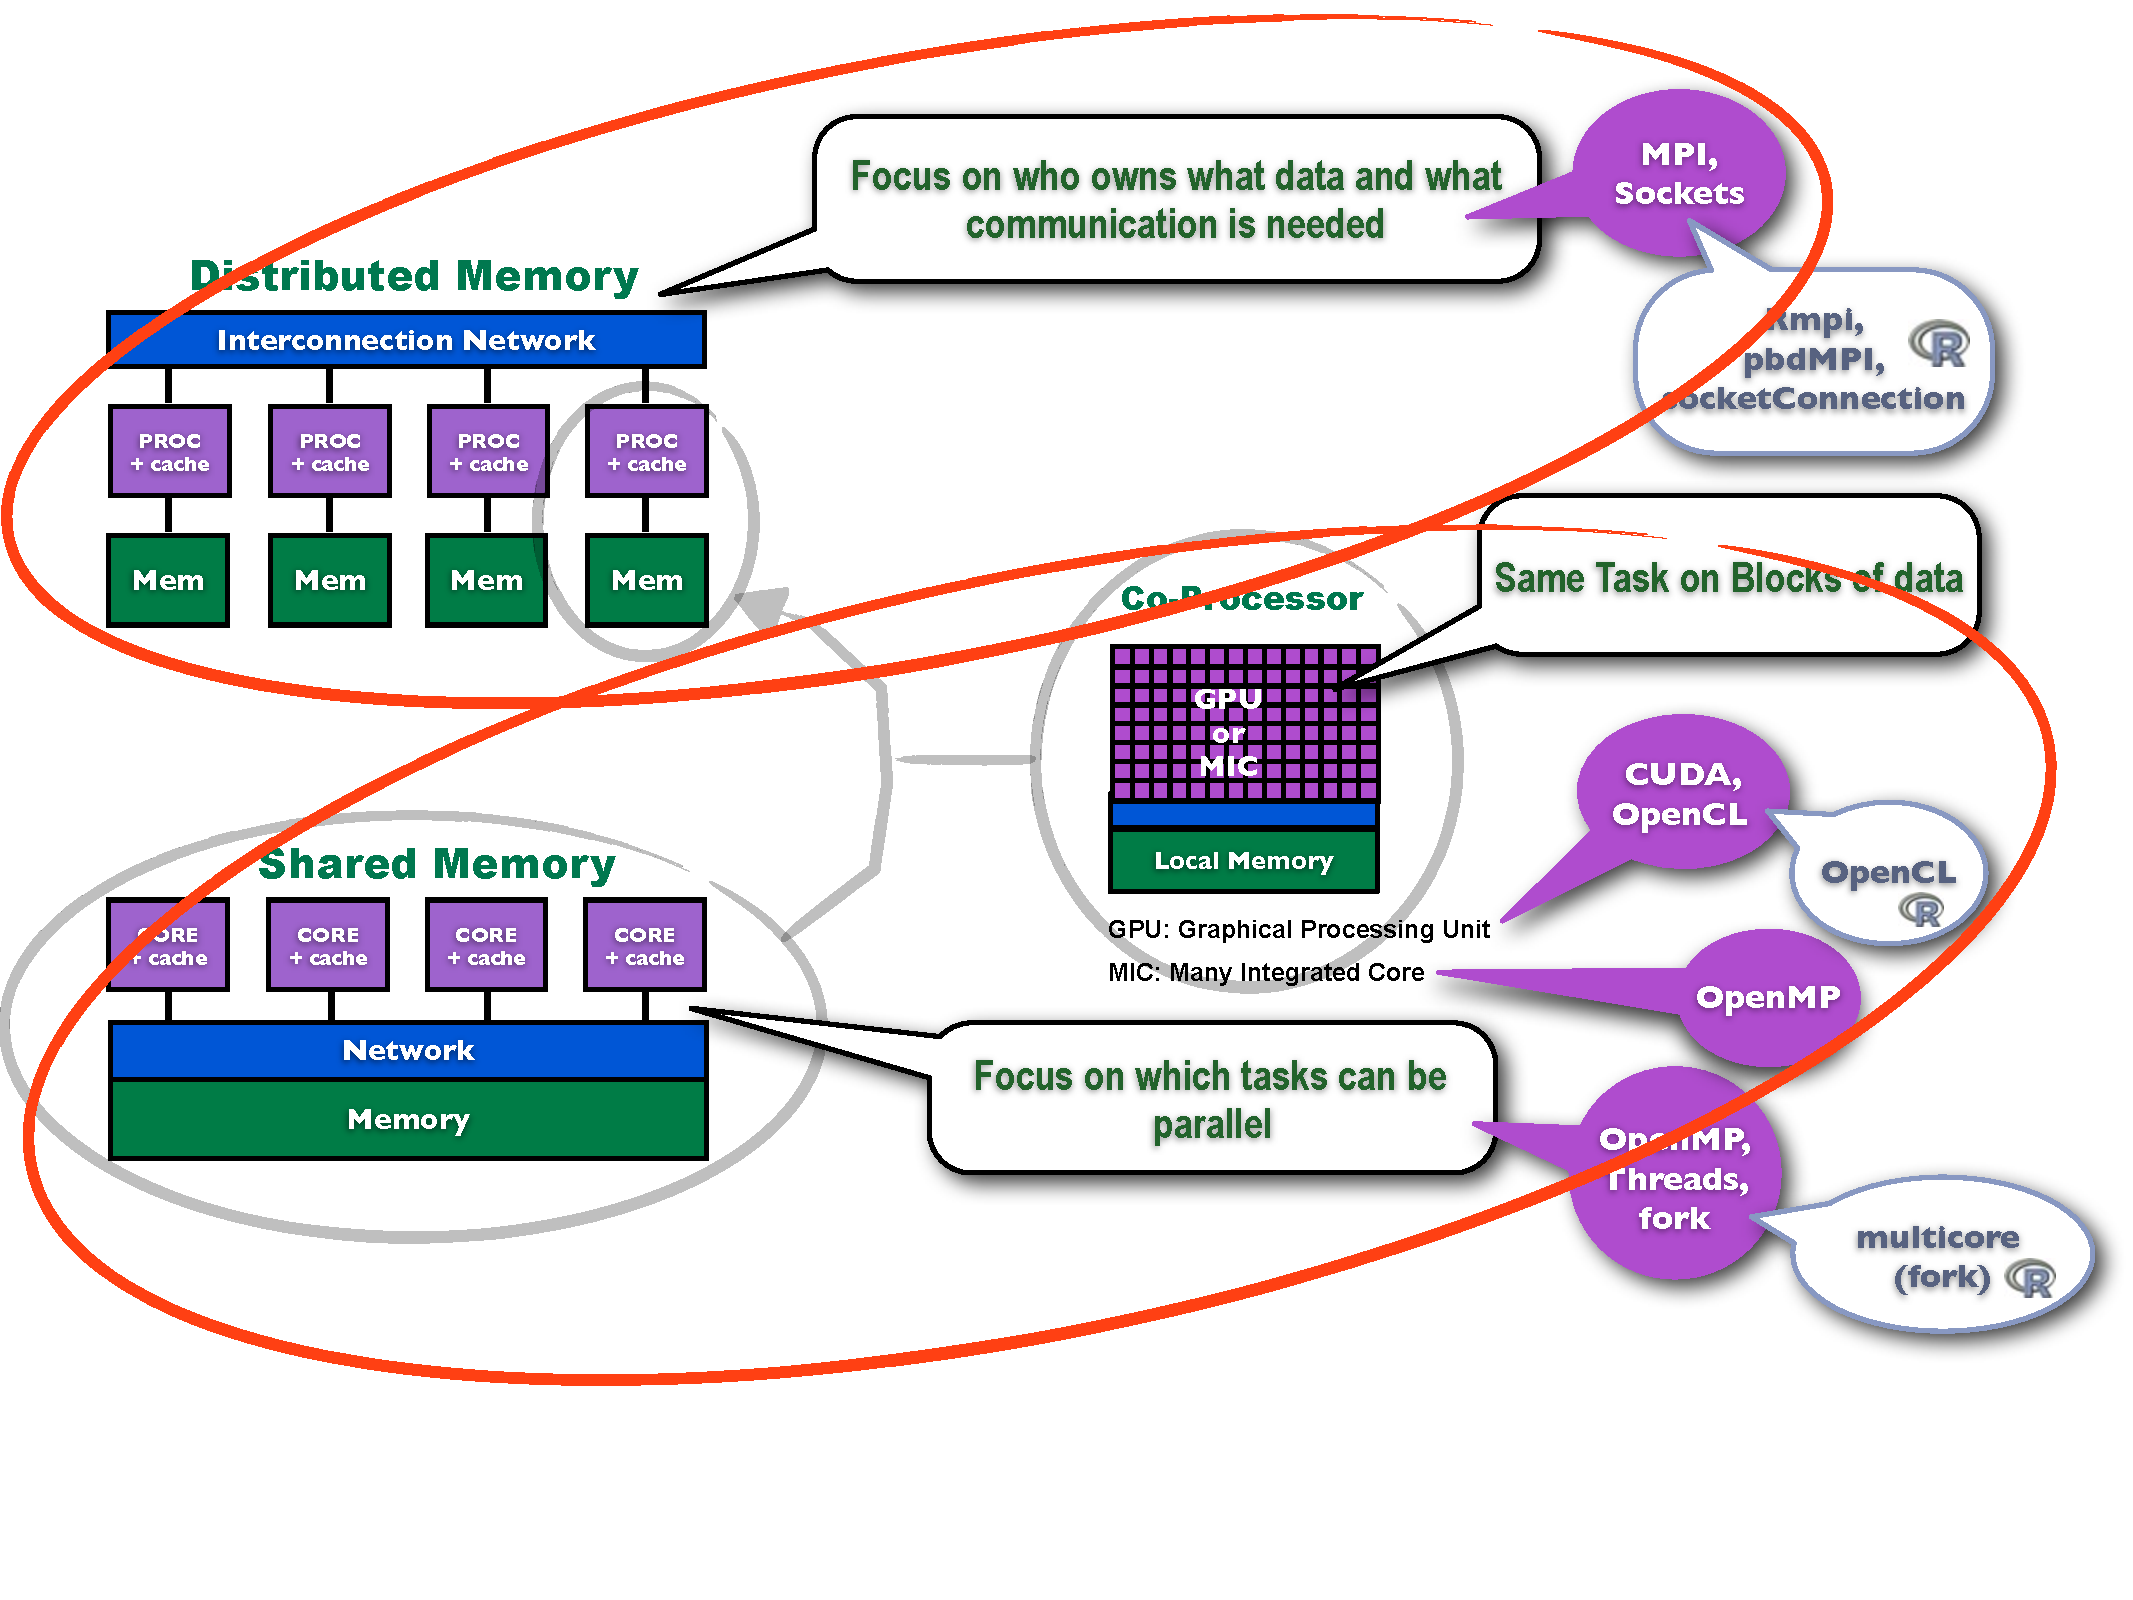
\includegraphics[width=0.95\textwidth]
{../common/pics/hardware/ParallelHardware10.pdf}
\end{frame}

% \begin{frame}{R and \pbdR Interfaces to HPC Libraries}
% \includegraphics[height=\textheight]
% {../common/pics/hardware/ParallelHardware26.pdf}
% \end{frame}

\begin{frame}{Parallel Programming Packages for R}
  \begin{block}{CRAN HPC Task View}\small
    \url{http://cran.r-project.org/web/views/HighPerformanceComputing.html}
  \end{block}
  \begin{center}
    \begin{block}{Shared Memory}
      \pkg{parallel}, \pkg{foreach}
    \end{block}
    \begin{block}{Distributed works in Shared Memory}
      \pbdR: \pkg{pbdMPI}, \pkg{pbdDMAT} (\pkg{pbdSLAP} and
      \pkg{pbdBASE})
    \end{block}
  \end{center}
\end{frame}


% \begin{frame}
%   \begin{block}{Portability}
%      Many parallel R packages break on Windows
%     \centering
% Windows seg fault **************************XS
% %    \includegraphics[scale=.7]{pics/bsod-preview}
%   \end{block}
% \end{frame}


\subsection{The parallel Package}
\makesubcontentsslidessec

\begin{frame}
  \begin{block}{The parallel Package}
    \begin{itemize}
      \item Comes with R $\geq$ 2.14.0
      \item Has 2 disjoint interfaces.
    \end{itemize}
    \begin{center}
      $\pkg{parallel} \hspace{.2cm} = \pkg{snow} \hspace{.2cm} +
      \hspace{.2cm} \pkg{multicore}$
    \end{center}

  \end{block}
\end{frame}


% \begin{frame}
%   \begin{block}{The parallel Package: multicore}
%   \begin{center}
%     Operates on fork/join paradigm.
%     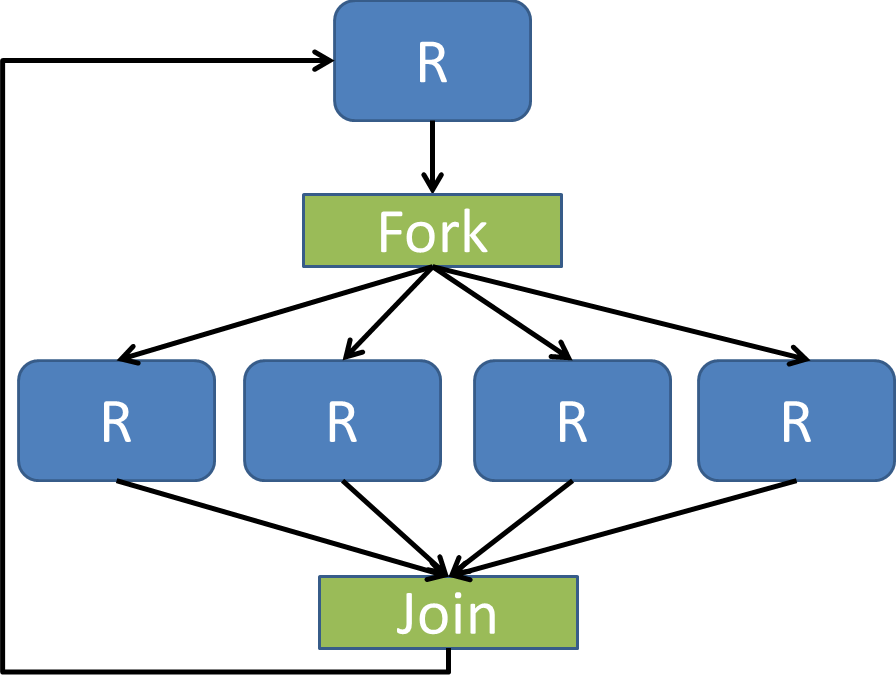
\includegraphics[scale=.35]{../common/pics/parallel/forkjoin}
%   \end{center}
%   \end{block}
% \end{frame}


\begin{frame}
  \begin{block}{The parallel Package: multicore}
    A simple Fork-Join parallel programming paradigm
    \begin{description}
    \item[+] Data copied to child on write (handled by OS)
    \item[+] Very efficient.
    \item[$-$] No Windows support.
    \item[$-$] Not as efficient as threads (C, C++, FORTRAN).
    \end{description}
  \end{block}
  \begin{center}
    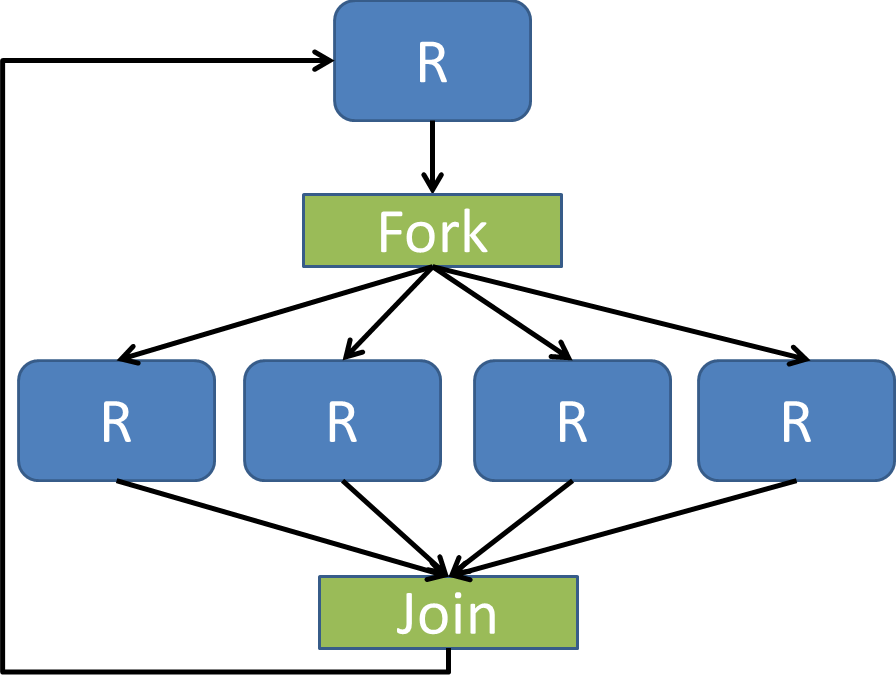
\includegraphics[scale=.20]{../common/pics/parallel/forkjoin}
  \end{center}
\end{frame}


\begin{frame}[fragile]
  \begin{block}{The parallel Package: multicore}
\begin{lstlisting}[language=sh]
mclapply(X, FUN, ...,
  mc.preschedule=TRUE, mc.set.seed=TRUE,
  mc.silent=FALSE, mc.cores=getOption("mc.cores", 2L),
  mc.cleanup=TRUE, mc.allow.recursive=TRUE)
\end{lstlisting}
\begin{lstlisting}
x <- lapply(1:10, sqrt)

library(parallel)
x.mc <- mclapply(1:10, sqrt)

all.equal(x.mc, x)
# [1] TRUE
\end{lstlisting}
  \end{block}
\end{frame}



\begin{frame}[fragile]
  \begin{block}{The parallel Package: multicore}
\begin{lstlisting}
unlist(mclapply(1:10, function(i) Sys.getpid(), mc.cores=4))
# [1] 13390 13391 13392 13393 13390 13391 13392 13393 13390 13391

unlist(mclapply(1:10, function(i) Sys.getpid(), mc.cores=2))
# [1] 13394 13395 13394 13395 13394 13395 13394 13395 13394 13395
\end{lstlisting}
  \end{block}
Check process id's involved.
\end{frame}


\begin{frame}
  \begin{block}{The parallel Package: snow}
    \begin{description}
      \item[?] Uses sockets.
      \item[+] Works on all platforms.
      \item[$-$] More fiddly than \code{mclapply()}.
      \item[$-$] Not as efficient as forks.
    \end{description}
  \end{block}
\end{frame}


\begin{frame}[fragile]
  \begin{block}{The parallel Package: snow}
\begin{lstlisting}
### Set up the worker processes
cl <- makeCluster(detectCores())
cl
# socket cluster with 4 nodes on host ‘localhost’

parSapply(cl, 1:5, sqrt)

stopCluster(cl)
\end{lstlisting}
  \end{block}
\end{frame}



\begin{frame}{The parallel Package: Summary}
  \begin{block}{All}
    \begin{itemize}
      \item \code{detectCores()}
      \item \code{splitIndices()}
    \end{itemize}
  \end{block}
  \begin{minipage}[t]{.475\textwidth}
    \begin{block}{multicore}
      \begin{itemize}
        \item \code{mclapply()}
        \item \code{mcmapply()}
        \item \code{mcparallel()}
        \item \code{mccollect()}
        \item and others\dots
      \end{itemize}
    \end{block}
  \end{minipage}
  \hfill
  \begin{minipage}[t]{.475\textwidth}
    \begin{block}{snow}
      \begin{itemize}
        \item \code{makeCluster()}
        \item \code{stopCluster()}
        \item \code{parLapply()}
        \item \code{parSapply()}
        \item and others\dots
      \end{itemize}
    \end{block}
  \end{minipage}
\end{frame}


\subsection{The foreach Package}
\makesubcontentsslidessec

\begin{frame}
  \begin{block}{The foreach Package}
    \begin{itemize}
    \item On Cran (Revolution Analytics).
    \item \pkg{foreach} is a single interface for a number of
      ``backend'' packages.
    \item Backends:  \pkg{doMC}, \pkg{doMPI}, \pkg{doParallel}, \pkg{doRedis},
      \pkg{doRNG}, \pkg{doSNOW}.
    \item A Manager-Workers approach
    \end{itemize}
  \end{block}
\end{frame}


\begin{frame}
  \begin{block}{The foreach Package}
    The Idea: Unify the disparate interfaces.
    \begin{itemize}
      \item[+] Works on all platforms (if backend does).
      \item[+] Can even work serial with minor notational change.
      \item[+] Write the code once, use whichever backend you prefer.
      \item[$-$] Binary operator, non-R-ish synatx.
      \item[$-$] Overhead issues if you aren't careful!
    \end{itemize}
  \end{block}
\end{frame}


\begin{frame}[fragile]{Overhead Issues}
\vspace{-.4cm}\hspace{-.6cm}
  \begin{minipage}[t]{.55\textwidth}
    \begin{center}
      \includegraphics[scale=.4]{../common/pics/parallel/parlogtimes}
    \end{center}
  \end{minipage}
  \hspace{.1cm}
  \begin{minipage}[t]{.45\textwidth}
\begin{lstlisting}
### Bad performance
foreach(i=1:len) %dopar% tinyfun(i)

### Expected performance
foreach(i=1:ncores) %dopar% {
  out <- numeric(len/ncores)
  for (j in 1:(len/ncores))
    out[i] <- tinyfun(j)
  out
}
\end{lstlisting}
  \end{minipage}
\end{frame}


\begin{frame}
  \begin{block}{The foreach Package: General Procedure}
    \begin{itemize}
      \item Load \pkg{foreach} and your backend package.
      \item Register your backend.
      \item Call \code{foreach}
    \end{itemize}
  \end{block}
\end{frame}


\begin{frame}[fragile]{Using foreach}
  \begin{minipage}{0.47\textwidth}
     Serial
      \begin{lstlisting}[escapeinside={(*@}{@*)}]
library(foreach)




### Example 1
foreach(i=1:3) (*@\textcolor{red}{\%do\%}@*) sqrt(i)

### Example 2
n <- 50
reps <- 100

x <- foreach(i=1:reps) (*@\textcolor{red}{\%do\%}@*) {
  sum(rnorm(n, mean=i)) / (n*reps)
}
      \end{lstlisting}
  \end{minipage}
  \hspace{-1ex}
  \begin{minipage}{0.52\textwidth}
    Parallel
      \begin{lstlisting}[escapeinside={(*@}{@*)}]
library(foreach)
library(<mybackend>)

register<MyBackend>()

### Example 1
foreach(i=1:3) (*@\textcolor{red}{\%dopar\%}@*) sqrt(i)

### Example 2
n <- 50
reps <- 100

x <- foreach(i=1:reps) (*@\textcolor{red}{\%dopar\%}@*) {
  sum(rnorm(n, mean=i)) / (n*reps)
}
      \end{lstlisting}
  \end{minipage}
\end{frame}


\begin{frame}[fragile]{foreach backends}
\begin{lstlisting}[title=multicore,escapeinside={(*@}{@*)}]
library(doParallel)
registerDoParallel(cores=ncores)
foreach(i=1:2) %dopar% Sys.getpid()
\end{lstlisting}

\begin{lstlisting}[title=snow,escapeinside={(*@}{@*)}]
library(doParallel)
cl <- makeCluster(ncores)
registerDoParallel(cl=cl)

foreach(i=1:2) %dopar% Sys.getpid()
stopCluster(cl)
\end{lstlisting}
\end{frame}


\begin{frame}
  \begin{block}{foreach Summary}
    \begin{itemize}
      \item Make sure to register your backend.
      \item Different backends may have different performance.
      \item Use \code{\%dopar\%} for parallel foreach.
      \item \code{\%do\%} and \code{\%dopar\%} \emph{must} appear on the same
line as the \code{foreach()} call.
    \end{itemize}
  \end{block}
\end{frame}

